\chapter{Third Party Tools and Resources}

\graphicspath{{../img/ch30/}}


In our solution we have exploited several tools and formalisms. These can be divided into two groups: linguistics and (inductive) logic programming. First we describe the linguistic tools and formalisms, the rest will follow.

\section{Linguistics Analysis} \label{sec:ch30_ling_tools}


\subsection{Prague Dependency Treebank (PDT)}

\begin{figure}
\centerline{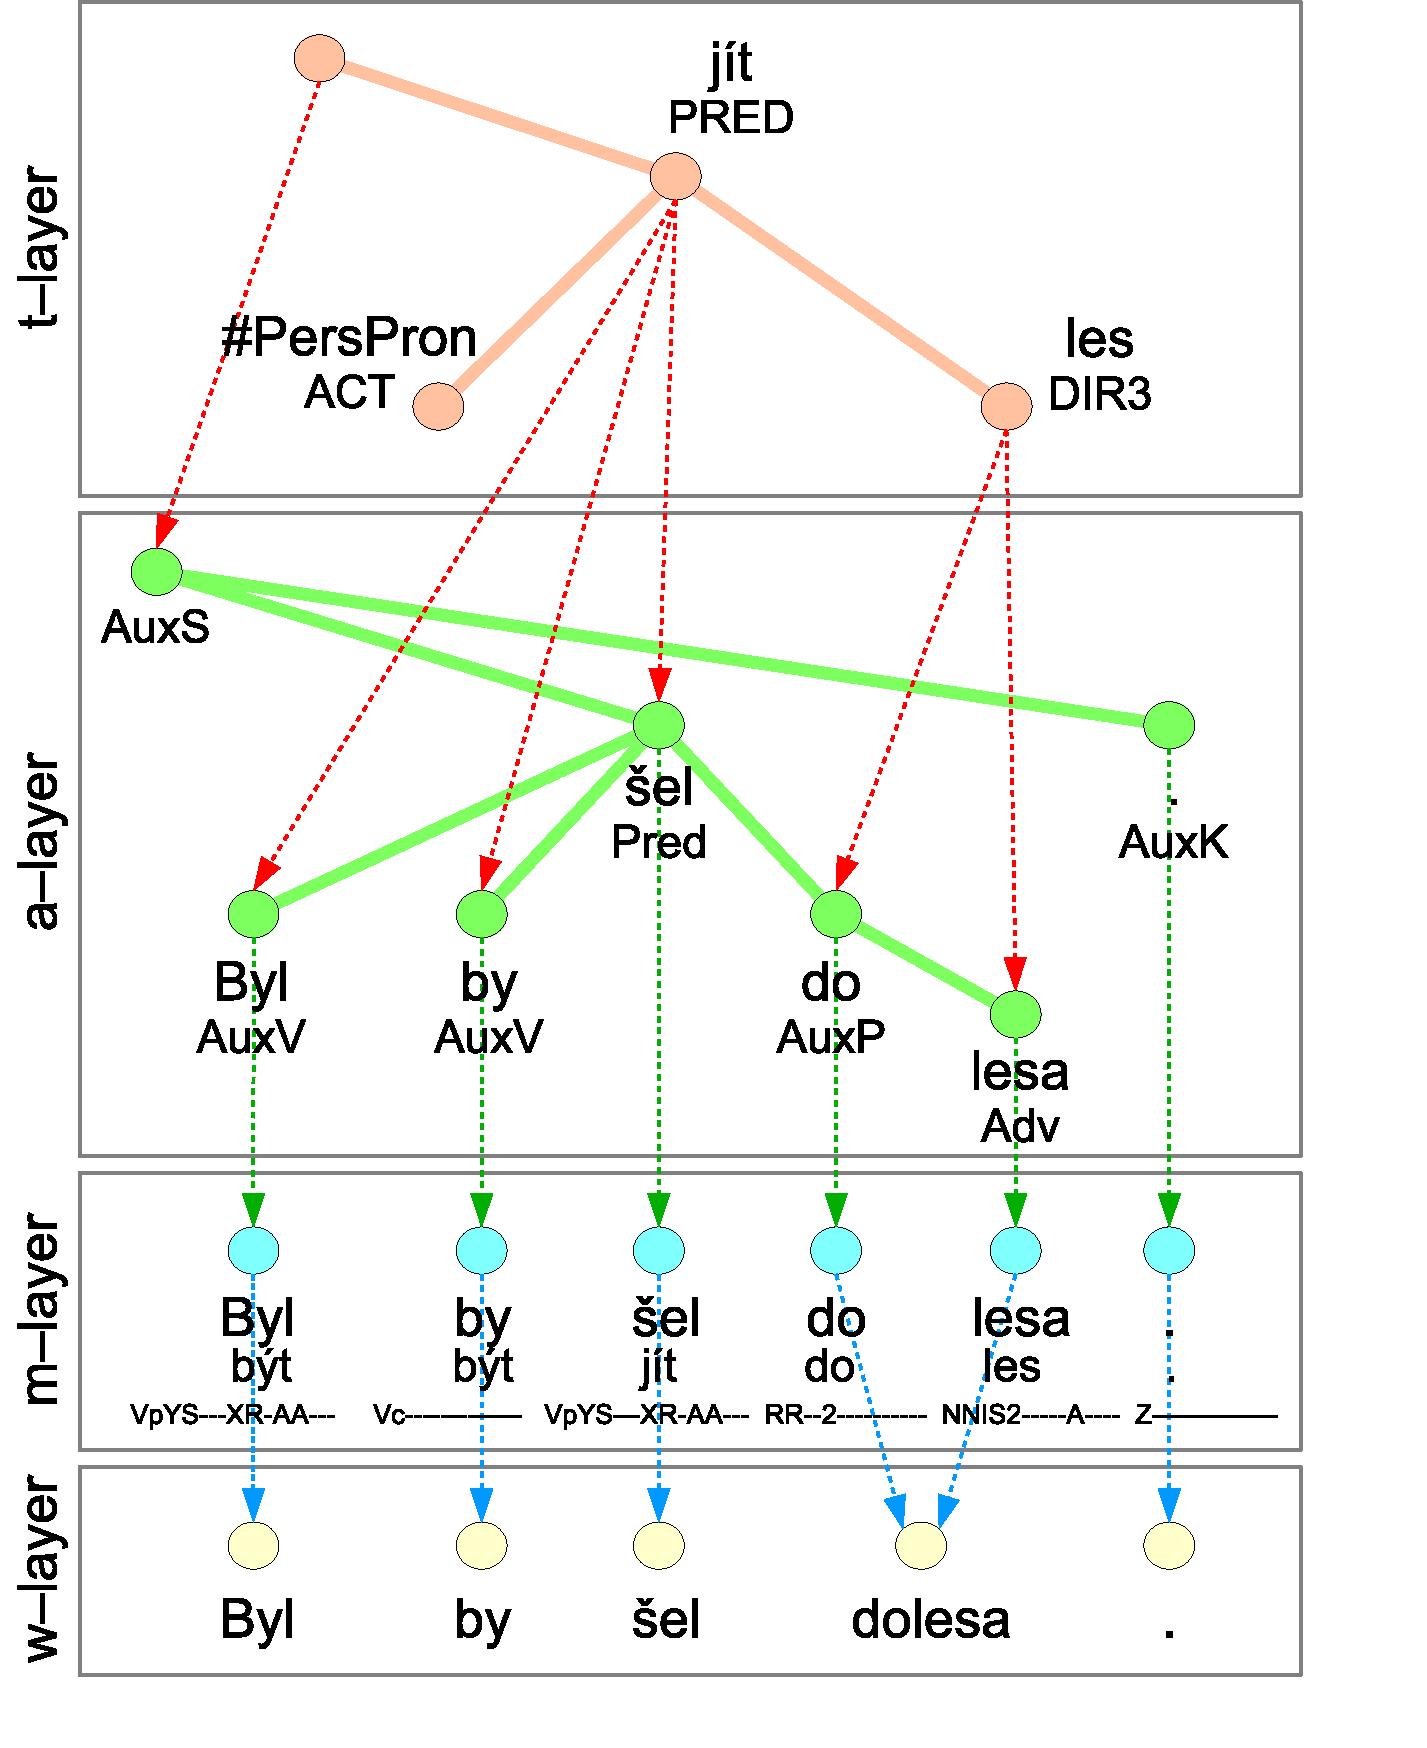
\includegraphics[width=0.6\hsize]{PDT_layers}}
\caption{Layers of linguistic annotation in PDT}
\label{fig:ch30_layers}
\end{figure}


\begin{itemize}
	\item Tectogrammatical layer
	\item Analytical layer
	\item Morphological layer
\end{itemize}

Byl by �el dolesa.
\\He-was would went toforest.


%%%%%%%%%%%%%%%%%%%%%%%%%%%%%%%%%%%%%%%%%%%%%%%%%%%%%%%%%%%%%%%%%%%%%%%%%%%%%%%%%%%%%%%%%%%%%%%%%
\subsubsection{Linguistic Analysis}
%%%%%%%%%%%%%%%%%%%%%%%%%%%%%%%%%%%%%%%%%%%%%%%%%%%%%%%%%%%%%%%%%%%%%%%%%%%%%%%%%%%%%%%%%%%%%%%%%

In this section we will briefly describe the linguistic tools that we have used to produce linguistic annotations of texts. These tools are being developed in the Institute of Formal and Applied Linguistics in Prague, Czech Republic. They are publicly available -- they have been published on a CDROM under the title PDT 2.0 (\cite{dedek:PDT20_CD} -- the first five tools) and in (\cite{dedek:KlTransformationBasedTectogrammatical2006} -- Tectogrammatical analysis). These tools are used as a processing chain. At the end of the chain they produce tectogrammatical dependency trees \citep{dedek:MiBeAnnotationtectogrammatical2006} built up from the text.


\begin{description}
 
	\item[Tool 1.] Segmentation and tokenization consists of dividing the input text into words and punctuation (tokenization) and dividing a sequence of tokens into sentences (segmentation).

	\item[Tool 2.] Morphological analysis assigns all possible lemmas and morphological tags to particular word forms (word
occurrences) in the text.

	\item[Tool 3.] Morphological tagging consists in selecting a single pair lemma-tag from all possible alternatives assigned
by the morphological analyzer.

	\item[Tool 4.] Collins' parser -- Czech adaptation. Unlike the usual approaches to the description of
English syntax, the Czech syntactic descriptions are dependency-based, which means that every edge of a syntactic tree captures the relation of dependency between a governor and its dependent node. Collins' parser gives the most probable parse of a given input sentence.

	\item[Tool 5.] Analytical function assignment assigns a description (analytical function, in linguistic sense) to every edge in the syntactic (dependency) tree.

	\item[Tool 6.] Tectogrammatical analysis produces linguistic annotation at the tectogrammatical level, sometimes called ``layer of deep syntax''. An example of a tectogrammatical tree can be seen in
Fig.~\ref{img:ch80_tree}. Annotation of a sentence at this layer is closer to the meaning of the sentence than its syntactic annotation; thus, information captured at the tectogrammatical layer is crucial for machine understanding of natural language \citep{dedek:KlTransformationBasedTectogrammatical2006}.
\end{description}





\subsubsection{Prague Markup Language (PML)}
\subsubsection{Feature Structure (FS)}


\subsection{Netgraph}

\subsection{Tree Editor TrEd (Btred)}

\subsection{TectoMT}
As we have started with our native language -- Czech (a language with rich morphology and free word order), we had to make tools for processing Czech available in GATE. We have implemented a wrapper for the TectoMT system\footnote{\url{http://ufal.mff.cuni.cz/tectomt/}} \citep{dedek:ZaPtTectoMTHighly2008} to GATE. TectoMT is a Czech project that contains many linguistic analyzers for different languages including Czech and English. We have used a majority of applicable tools from TectoMT: a tokeniser, a sentence splitter, morphological analyzers (including POS tagger), a syntactic parser and the deep syntactic (tectogrammatical) parser. All the tools are based on the dependency based linguistic theory and formalism of the Prague Dependency Treebank project \citep{dedek:PDT20_CD}. So far our solution does not include any coreference and discourse analysis.


%Czech language
%\\Slavic language, with rich morphology, free word order
%\\Stanford dependencies

\subsection{Czech WordNet}

The Figure~\ref{img:extract_patern} shows, that it would be useful to gather words with similar meanings in our extraction rules. For example, the rule in the Figure~\ref{img:extract_patern} contains long disjunctions of similar words (nodes with numbers 1 and 4). These disjunctions could be replaced with some kind of expression telling that we are looking for any word from some semantic category (e.g. human beings). For this purpose we wanted to use the Czech WordNet \citep{biblio:WordNetCZ2004}. 

After we have explored the records of the Czech WordNet (CzWN) related to the domain of our interest (car accidents, etc.) we have decided not to involve CzWN in the extraction process. The reason is that the coverage of the vocabulary of our domain is rather poor and the semantic connections of words are sometimes unfortunately missing. But we can supply the missing information to CzWN or we can build up a new domain-specific word-net based on the ground of CzWN.  



\subsection{GATE}
GATE\footnote{\url{http://gate.ac.uk/}} \citep{dedek:GATE_ACL2002} is probably the most widely used tool for text processing. In our solution the capabilities of document and annotation management, utility resources for annotation processing, JAPE grammar rules \citep{Cunningham00jape:a}, machine learning facilities and performance evaluation tools are the most helpful features of GATE that we have used.



\section{Weka}


\section{Inductive Logic Programming}
Inductive Logic Programming (ILP) \citep{dedek:MuggletonILP} is a machine learning technique based on logic programming. Given an encoding of the known background knowledge (in our case linguistic structure of all sentences) and a set of examples represented as a logical database of facts (in our case tokens annotated with the target annotation type are positive examples and the remaining tokens negative ones), an ILP system will derive a hypothesized logic program (in our case extraction rules) which entails all the positive and none of the negative examples.

\subsection{ILP tool}
As an ILP tool we have used ``A Learning Engine for Proposing Hypotheses'' (Aleph v5)\footnote{\url{http://www.comlab.ox.ac.uk/activities/machinelearning/Aleph/}}, which we consider very practical. It uses quite effective method of inverse entailment \citep{biblio:InverseEntailment} and keeps all handy features of a Prolog system (we have used YAP Prolog\footnote{\url{http://www.dcc.fc.up.pt/~vsc/Yap/}}) in its background.


From our experiments (Section~\ref{sec:evaluation}) can be seen that ILP is capable to find complex and meaningful rules that cover the intended information.



\textbf{?? large amount of training data ??}

As we do not have large amount of training data, there is no problem with excessive time demands during learning and the application of the learned rules is simple and quick.



